\documentclass[a4paper]{article}
    \usepackage[UTF8]{ctex}
    \usepackage{amsmath,amsthm,amssymb}

    \usepackage{minted}
    \usepackage{xcolor}
    \usepackage[colorlinks,linkcolor=red,anchorcolor=blue,citecolor=green]{hyperref}
    \usepackage[margin=1in]{geometry}
    \usepackage{caption}
    \usepackage{graphicx}
    \usepackage{subfigure}
    \usepackage{float}
    \usepackage{fontspec}
    \usepackage{booktabs}
    \setmainfont{Times New Roman}
    \setmonofont{Consolas}
    \definecolor{bg}{rgb}{0.9,0.9,0.9}
    \usemintedstyle{manni}
    \setminted{
    linenos,
    autogobble,
    breaklines,
    breakautoindent,
    bgcolor=bg,
    numberblanklines=false,
    }

\begin{document}
    \begingroup
    \hypersetup{linkcolor=black}
    \tableofcontents
    \endgroup
    \newpage
    \section{实验介绍}
        \subsection{实验内容}
在dataset文件夹中的所有图片中搜索target.jpg图片所示物体,并绘制程序认为的好的匹配.
        \subsection{实验环境}
操作系统: Ubuntu 18.04 LTS

Python版本: 3.7

NumPy: 1.14.5

OpenCV-Python: 3.4.3.18
    \newpage
    \section{实验过程}
        \subsection{SIFT图像特征提取原理}
尺度不变特征变换(Scale-Invariant Feature Transform, SIFT), 是计算机视觉领域的一种图像特征检测算法,用于检测并描述
图像的局部特征. 该算法于1999年由David Lowe提出, 并广泛应用于计算机视觉的诸个领域.

SIFT算法基于图像的局部特征,可以很好地处理图像的匹配问题,具有如下特点:

1.SIFT特征是图像的局部特征,其对旋转、尺度缩放、亮度变化保持不变性,对视角变化、仿射变换、噪声也保持一定程度的稳定性;

2.独特性好,信息量丰富,适用于在海量特征数据库中进行快速、准确的匹配;

3.多量性,即使少数的几个物体也可以产生大量的SIFT特征向量;

4.高速性,经优化的SIFT匹配算法甚至可以达到实时的要求;

5.可扩展性,可以很方便的与其他形式的特征向量进行联合.

SIFT图像特征提取有4个基本步骤,分别为:

1.尺度空间极值点检测

2.关键点精确定位

3.关键点方向确定

4.关键点描述子生成
        \subsection{尺度空间极值点检测}
此步骤中,对图像建立了尺度空间,实现时使用高斯差分金字塔来表示,然后寻找高斯差分(DoG)空间中的局部极值点.

由于本次实验并未深入此步骤,故在此略去具体实现细节.
        \subsection{关键点精确定位}
上一步中所检测到的极值点是离散空间的极值点,并不是真正的极值点,因而需要在这一步骤中进行更加精确的定位.根据SIFT算法的原理,需要对
尺度空间的DoG函数进行曲线拟合(利用其在尺度空间的Taylor展开式);同时,还需要进一步消除位于边缘处的关键点(利用关键点处的Hessian矩阵).

同样地,本次实验并未深入于此,故在此略过.
        \subsection{关键点方向确定}
在经过前两个步骤的处理后,我们得到了图像中一定数量的关键点坐标.

当然,需要说明的是,本次实验中简便起见,我们调用OpenCV提供的函数,直接获取图像中的Shi-Tomasi角点.Shi-Tomasi 角点检测算法,是J.Shi和
C.Tomasi于1994年所提出的一种对Harris角点检测算子的改进.
\begin{minted}{python}
img = cv2.imread(image_path)
img = rgb_to_grayscale(img)
shi_tomasi_corners = cv2.goodFeaturesToTrack(img, maxCorners=50, qualityLevel=0.01, minDistance=10)
# reshape into (N,2)
shi_tomasi_corners = shi_tomasi_corners.reshape((-1, 2)).astype("int32")

\end{minted}

那么,对于检测到的每一个关键点,我们计算其$16\times16$邻域内像素点的梯度强度与方向.然后将$0 - 2\pi$的范围等分为36个区间,统计
这$16\times16$个像素点的梯度方向分布(以其梯度强度为权值).最终,我们选取权重最大的区间的中值作为该关键点的主方向.

在具体的编程实现中,为避免梯度的重复计算,同时简化代码,我采取了一次性计算整幅图像像素点梯度的方法.需要注意的是,使用\mintinline{python}
{np.arctan()}函数计算得到的方向范围为$-\pi /2  -  \pi /2$,为了得到$0  -  2\pi$范围,需要根据梯度的$x,y$方向分量符号进行判断:
\begin{minted}{python}
def compute_gradient(grayscale_image):
    img = grayscale_image.copy().astype("int32")
    gradient, direction = [np.zeros_like(img, dtype="float32"), ] * 2
    width, height = img.shape
    for i in range(width - 1):  # just ignore pixels on the edge
        for j in range(height - 1):
            d_x = img[i+1, j] - img[i-1, j]
            d_y = img[i, j+1] - img[i, j-1]
            gradient[i][j] = np.sqrt(d_x * d_x + d_y * d_y)
            direction[i][j] = np.arctan(d_y/(d_x + 1e-8))   # -pi/2 ~ pi/2
            if(d_x < 0):
                direction[i][j] += np.pi    # -pi/2 ~ 3pi/2
            if(direction[i][j] < 0):
                direction[i][j] += 2 * np.pi
    return gradient, direction
\end{minted}

而在计算关键点的主方向时,需要考虑到关键点靠近图片边沿的特殊情形,避免选取的关键点邻域超出图像的有效范围:
\begin{minted}{python}
def vote_for_direction(gradient_zone, direction_zone):
    potential_directions = np.zeros((36,))
    width, height = gradient_zone.shape
    for i in range(0, width):
        for j in range(0, height):
            d = int(direction_zone[i][j] // (np.pi/18))
            potential_directions[d] += gradient_zone[i][j]
    direction = (np.argmax(potential_directions) + 0.5) * np.pi / 18
    return direction
width, height = gradient.shape
x1, x2, y1, y2 = max(0, x-8), min(width, x+8), max(0, y-8), min(height, y+8)
main_direction = vote_for_direction(
    gradient[x1:x2, y1:y2], direction[x1:x2, y1:y2])
\end{minted}
        \subsection{关键点描述子生成}
在得到关键点的主方向$\theta_0$之后,SIFT算法将其作为物体坐标系的X方向,那么对于关键点$16\times16$邻域范围内的所有像素点的梯度,需要将
其从原先的图像坐标系换算到物体坐标系中:
$$\theta^{'}(x,y) = \theta(x,y) - \theta_0$$

这一步操作使得SIFT算法能够较好地处理图片的旋转变换,具有旋转不变性.

然而,在进行坐标系换算之后,物体坐标系上的点对应的图像坐标系上的点坐标可能并不是整数,因而需要插值处理,在这里我采用了双线性插值法,即:
$$\theta(x^{'} , y^{'}) = \theta(x,y)dx_2 dy_2 + \theta(x+1,y)dx_1 dy_2 + \theta(x,y+1)dx_2 dy_1
+ \theta(x+1,y+1)dx_1 dy_1$$
\begin{figure}[H]
\centering

\includegraphics[width=.6\textwidth]{img/1.png}
\caption{插值法}
\end{figure}
编程实现如下:
\begin{minted}{python}
def get_gradient(gradient, x, y):  # x,y might not be integers
    x_low, x_high = int(x), int(x)+1
    y_low, y_high = int(y), int(y)+1
    result = gradient[x_low][y_low] * (x_high - x) * (y_high - y)
    result += gradient[x_low][y_high] * (x_high - x)*(y-y_low)
    result += gradient[x_high][y_low] * (x-x_low) * (y_high - y)
    result += gradient[x_high][y_high] * (x-x_low) * (y - y_low)
    return result

def get_adjusted_direction(direction, main_direction, x, y):
    x_low, x_high = int(x), int(x)+1
    y_low, y_high = int(y), int(y)+1
    result = direction[x_low][y_low] * (x_high - x) * (y_high - y)
    result += direction[x_low][y_high] * (x_high - x)*(y-y_low)
    result += direction[x_high][y_low] * (x-x_low) * (y_high - y)
    result += direction[x_high][y_high] * (x-x_low) * (y - y_low)
    result -= main_direction
    if result < 0:
        result += 2*np.pi
    return result
\end{minted}

在获取了物体坐标系中$16\times16$邻域所有点的梯度强度与方向之后,则可据此生成该关键点的SIFT描述子: 将$16\times16$的邻域均分成
$4\time4$个块,每块有$4\times4$个像素点.而在每个块内,类似于求主方向,把$0-2\pi$等分为8个区间,统计梯度直方图,从而得到
维度为8的直方图向量. 因此,对于每个关键点,最终生成了$4\times4\times8 = 128$维的SIFT描述子.额外地,在生成了描述子之后,
需要对其归一化处理,以便后续的匹配.
\begin{minted}{python}
def extract_features(gradient, direction):  # both input size 16*16

    def compute_histogram(x, y):  # [x,x+3]*[y,y+3]
        bins = np.zeros((8,))
        for i in range(x, x+4):
            for j in range(y, y+4):
                d = int(direction[i][j] // (np.pi/4))
                bins[d] += gradient[i][j]
        return bins

    assert gradient.shape == (16, 16), "Invalid shape!"
    features = list()
    for i in range(0, 13, 4):
        for j in range(0, 13, 4):
            features.append(compute_histogram(i, j))
    features = np.array(features).reshape((-1,))
    features = features / np.sqrt(np.sum(features * features))
    return features
\end{minted}

        \subsection{相似图片匹配}
给定一张图片,根据以上算法,对其提取出N个128维SIFT描述子,那么,检测两张图片是否相似,可以通过检测两者的SIFT描述子是否相似来
初步实现.

对于两个SIFT描述子,由于我们已经对其做过归一化处理,那么比较其相似度,只需计算二者在向量空间中的夹角大小,或是直接
计算二者的向量内积.当二者的内积超过一定的阈值,我们便认为二者成功匹配,否则失败.

在编程实现中,对于一个描述子,先找到与其相似度最高的描述子,匹配成功后将其置零,以避免重复匹配.同时将位于\mintinline{python}
{feature[1],target_feature[1]}中的关键点坐标对保存.图片匹配结束后,返回匹配点个数\mintinline{python}{score}与匹配
关键点坐标对.

\begin{minted}{python}
def sift_match(target_feature, feature, threshold):
    score = 0
    result = list()
    for i, descriptor in enumerate(target_feature[1]):
        max_j, max_similarity = 0, 0
        for j, x in enumerate(feature[1]):
            if np.dot(descriptor, x) >= max_similarity:
                max_j, max_similarity = j, np.dot(descriptor, x)
        if max_similarity >= threshold:
            score += 1
            feature[1][max_j] = np.zeros_like(feature[1][max_j])
            result.append((target_feature[0][i], feature[0][max_j]))
    return score, result
\end{minted}

为了方便展示匹配结果,在找到最佳匹配图片之后,将其与目标图片并排列为一张新图片,同时将匹配点用线段相连,以便观察.

考虑到目标图片与最佳匹配图片的尺寸差异,在合并二者时,需要对其中尺寸较小者进行填充拓展(使用\mintinline{python}
{cv2.copyMakeBorder()}),使得二者高度相匹配.然而,这样做之后,
必须保存这两张图片的最左上角像素点在合并后图片的位置,否则将无法定位图片的关键点.

\begin{minted}{python}
def merge(img1, img2):
    result = []
    img1 = cv2.imread(img1)
    img2 = cv2.imread(img2)
    final_height = max(img1.shape[0], img2.shape[0])
    padding = int((final_height - img1.shape[0]) // 2)
    result.append(padding)
    result.append(padding)
    odd = 1 if padding * 2 != (final_height - img1.shape[0]) else 0
    img1 = cv2.copyMakeBorder(img1, padding, padding+odd, padding, padding, cv2.BORDER_CONSTANT, value=[0, 0, 0])
    padding = int((final_height - img2.shape[0]) // 2)
    result.append(padding+img1.shape[1])
    result.append(padding)
    odd = 1 if padding * 2 != (final_height - img2.shape[0]) else 0
    img2 = cv2.copyMakeBorder(img2, padding, padding+odd, padding, padding, cv2.BORDER_CONSTANT, value=[0, 0, 0])
    result.append(np.hstack((img1, img2)))
    return result
def link_matched_points(merged_img, x1, y1, x2, y2, match_result):
    new_img = merged_img.copy()
    cv2.circle(new_img, (x1, y1), 5, [0, 0, 255], -1)
    cv2.circle(new_img, (x2, y2), 5, [0, 0, 255], -1)
    for pair in match_result:
        cv2.line(new_img, (int(x1+pair[0][0]), int(y1+pair[0][1])), (int(x2+pair[1][0]), int(y2+pair[1][1])), [255, 0, 0], 2)
    return new_img

x1, y1, x2, y2, merged_img = merge(target_image, possible_images[best_match])
final_img = link_matched_points(merged_img, x1, y1, x2, y2, match_result[best_match][1])
\end{minted}
    \newpage
    \section{实验结果}
在经过尝试之后,设定角点检测数为50,SIFT描述子匹配阈值为0.6,对dataset文件中的5张图片与target.jpg进行匹配,实验结果如下:
(图片后的数字代表图像中成功匹配的关键点个数)
\begin{minted}{text}
dataset/1.jpg 9
dataset/2.jpg 13
dataset/3.jpg 17
dataset/4.jpg 11
dataset/5.jpg 12
The best match is:  dataset/3.jpg
\end{minted}

可见,利用SIFT算法,成功地从多张图片中找到了目标图像.那么,将最佳匹配图片与目标图片展示出来,结果如图\ref{result}所示.
\begin{figure}[H]
\centering
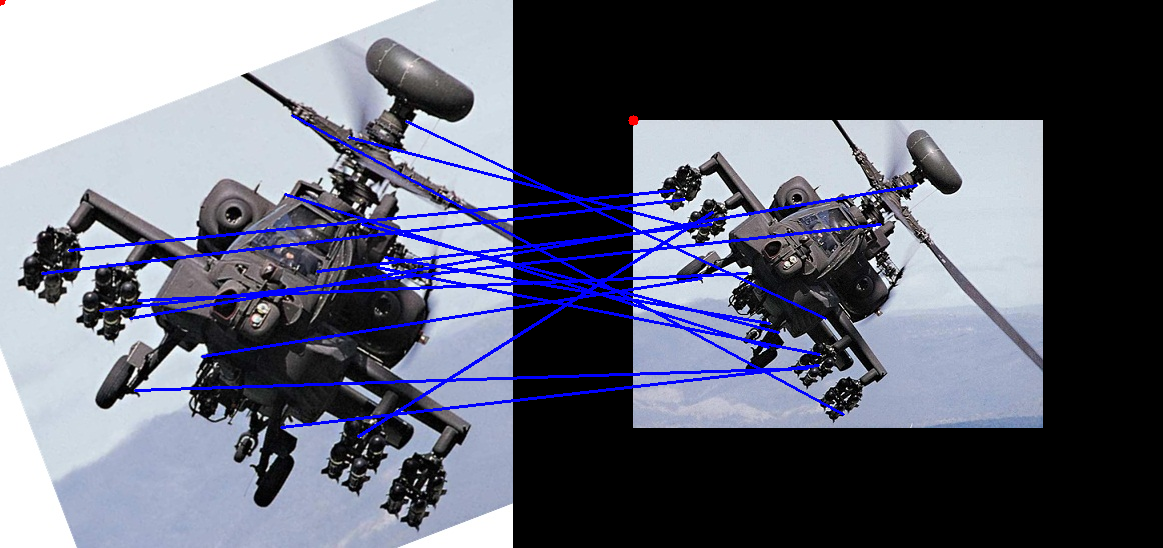
\includegraphics[width=.8\textwidth]{img/Result.png}
\caption{匹配结果}
\label{result}
\end{figure}
\newpage
\section{总结与分析}
在本次实验中,虽然并未对SIFT算法进行完整的实现,但通过查阅资料,加以实现SIFT算法生成描述子的部分,我对SIFT算法有了较深入
的理解.同时,在实验中,遇到了诸多实现上的细节问题,诸如邻域超出图片范围,这些问题在仅仅通过查看对SIFT算法的粗略描述往往难以
解决,需要根据自己的理解加以解决并多次尝试.

事实上,如果仔细观察两幅图片的匹配结果(图\ref{result}),会发现其实有一定数量的错误匹配存在.这些错误虽未影响最终的匹配结果,
但是也显出了我所实现的SIFT算法存在缺陷(甚至是错误).这些问题可能来源于我对一些细节的不当处理,也有可能是检测参数与阈值设置不当
……

总而言之,实现完整的SIFT算法并不容易,然而所幸的是,在一般的应用场合,我们可以直接调用OpenCV或是其他库包所提供的实现,从而避开
算法的繁冗细节.
\end{document}
